\documentclass[UTF8,a4paper,10pt]{ctexart}
\usepackage[left=2.00cm, right=2.00cm, top=3.50cm, bottom=3.50cm]{geometry} %页边距
\CTEXsetup[format={\Large\bfseries}]{section} %设置章标题居左
 
 
%%%%%%%%%%%%%%%%%%%%%%%
% -- text font --
% compile using Xelatex
%%%%%%%%%%%%%%%%%%%%%%%
% -- 中文字体 --
%\setmainfont{Microsoft YaHei}  % 微软雅黑
%\setmainfont{YouYuan}  % 幼圆    
%\setmainfont{NSimSun}  % 新宋体
%\setmainfont{KaiTi}    % 楷体
%\setmainfont{SimSun}   % 宋体
%\setmainfont{SimHei}   % 黑体
% -- 英文字体 --
%\usepackage{times}
%\usepackage{mathpazo}
%\usepackage{fourier}
%\usepackage{charter}
\usepackage{helvet}
\usepackage{amsmath, amsfonts, amssymb} % math equations, symbols
\usepackage[english]{babel}
\usepackage{color}      % color content
\usepackage{graphicx}   % import figures
\usepackage{subfig}
\usepackage{url}        % hyperlinks
\usepackage{bm}         % bold type for equations
\usepackage{multirow}
\usepackage{longtable}
\usepackage{booktabs}
\usepackage{epstopdf}
\usepackage{epsfig}
\usepackage{algorithm}
\usepackage{algorithmic} 
\usepackage{listings} 
\usepackage{xcolor}
\lstset{
    language=matlab,  %代码语言使用的是matlab
    frame=shadowbox, %把代码用带有阴影的框圈起来
    rulesepcolor=\color{red!20!green!20!blue!20},%代码块边框为淡青色
    keywordstyle=\color{blue!90}\bfseries, %代码关键字的颜色为蓝色,粗体
    commentstyle=\color{red!10!green!70}\textit,    % 设置代码注释的颜色
    showstringspaces=false,%不显示代码字符串中间的空格标记
    numbers=left, % 显示行号
    numberstyle=\tiny,    % 行号字体
    stringstyle=\ttfamily, % 代码字符串的特殊格式
    breaklines=true, %对过长的代码自动换行
    extendedchars=false,  %解决代码跨页时,章节标题,页眉等汉字不显示的问题
%   escapebegin=\begin{CJK*},escapeend=\end{CJK*},      
% 代码中出现中文必须加上,否则报错
    texcl=true}
\renewcommand{\algorithmicrequire}{ \textbf{Input:}}     % use Input in the format of Algorithm  
\renewcommand{\algorithmicensure}{ \textbf{Initialize:}} % use Initialize in the format of Algorithm  
\renewcommand{\algorithmicreturn}{ \textbf{Output:}}     % use Output in the format of Algorithm   

% -------------------------允许算法跨页-------------
\makeatletter
\newenvironment{breakablealgorithm}
    {% \begin{breakablealgorithm}
    \begin{center}
        \refstepcounter{algorithm}% New algorithm
        \hrule height.8pt depth0pt \kern2pt% \@fs@pre for \@fs@ruled
        \renewcommand{\caption}[2][\relax]{% Make a new \caption
            {\raggedright\textbf{\ALG@name~\thealgorithm} ##2\par}%
                \ifx\relax##1\relax % #1 is \relax
                    \addcontentsline{loa}{algorithm}{\protect\numberline{\thealgorithm}##2}%
                \else % #1 is not \relax
                    \addcontentsline{loa}{algorithm}{\protect\numberline{\thealgorithm}##1}%
                \fi
            \kern2pt\hrule\kern2pt
        }
  }{% \end{breakablealgorithm}
            \kern2pt\hrule\relax% \@fs@post for \@fs@ruled
        \end{center}
  }
\makeatother
 
\usepackage{fancyhdr} %设置页眉、页脚
%\pagestyle{fancy}
\lhead{}
\chead{}
%\rhead{\includegraphics[width=1.2cm]{fig/ZJU_BLUE.eps}}
\lfoot{}
\cfoot{}
\rfoot{}
%\pagestyle{empty} %删除所有页码
 
%%%%%%%%%%%%%%%%%%%%%%%
%  设置水印
%%%%%%%%%%%%%%%%%%%%%%%
%\usepackage{draftwatermark}         % 所有页加水印
%\usepackage[firstpage]{draftwatermark} % 只有第一页加水印
% \SetWatermarkText{Water-Mark}           % 设置水印内容
% \SetWatermarkText{\includegraphics{fig/ZJDX-WaterMark.eps}}         % 设置水印logo
% \SetWatermarkLightness{0.9}             % 设置水印透明度 0-1
% \SetWatermarkScale{1}                   % 设置水印大小 0-1    
 
\usepackage{hyperref} %bookmarks
\hypersetup{colorlinks, bookmarks, unicode} %unicode
 

\title{\textbf{并行单纯形法}}
\author{ 211840196 张博阳 }
\date{}

\begin{document}
\maketitle
\section{实现思路}
Richard Marciano, Teodor Rus在1988年就提出利用并行手段加快换基结束后迭代单纯形表的计算速度$^{[1]}$. 在2017年,  Péter Tar等提出了利用密集计算等方法对单纯形法进行并行加速, 其中对于凸多面体的顶点寻优问题, 从多个初始位置开始进行单纯形表迭代可以实现加速及更好的鲁棒性表现$^{[1]}$. 本项目从这两个方向分别进行单纯形法的并行化实现. 由于计算资源的有限, 仅对两种方法分别进行实现, 而无对进程分组的两种方法结合实现并行.
\section{代码框架及并行化手段}
项目类图如下.
\begin{figure*}[htbp]
    \centering
    \includegraphics[width=14cm]{MPI\_SimplexSolver.drawio.png}
\end{figure*}
\texttt{SimplexSolver}类为单线程下的单纯形法求解器类, 其中依赖\texttt{Matrix}和\texttt{Vector}两个工具类. 在\texttt{SimplexSolver}基础上扩展为\texttt{MPI\_SimplexSolver}, 其使用MPI接口对核心函数\texttt{solve()}实现并行. \texttt{IOHelper}为项目进行I/O操作的辅助类.
\par
\texttt{Matrix}类封装了二维数组和初等行变换等单纯形法需要的矩阵行为.
\begin{figure*}[htbp]
    \centering
    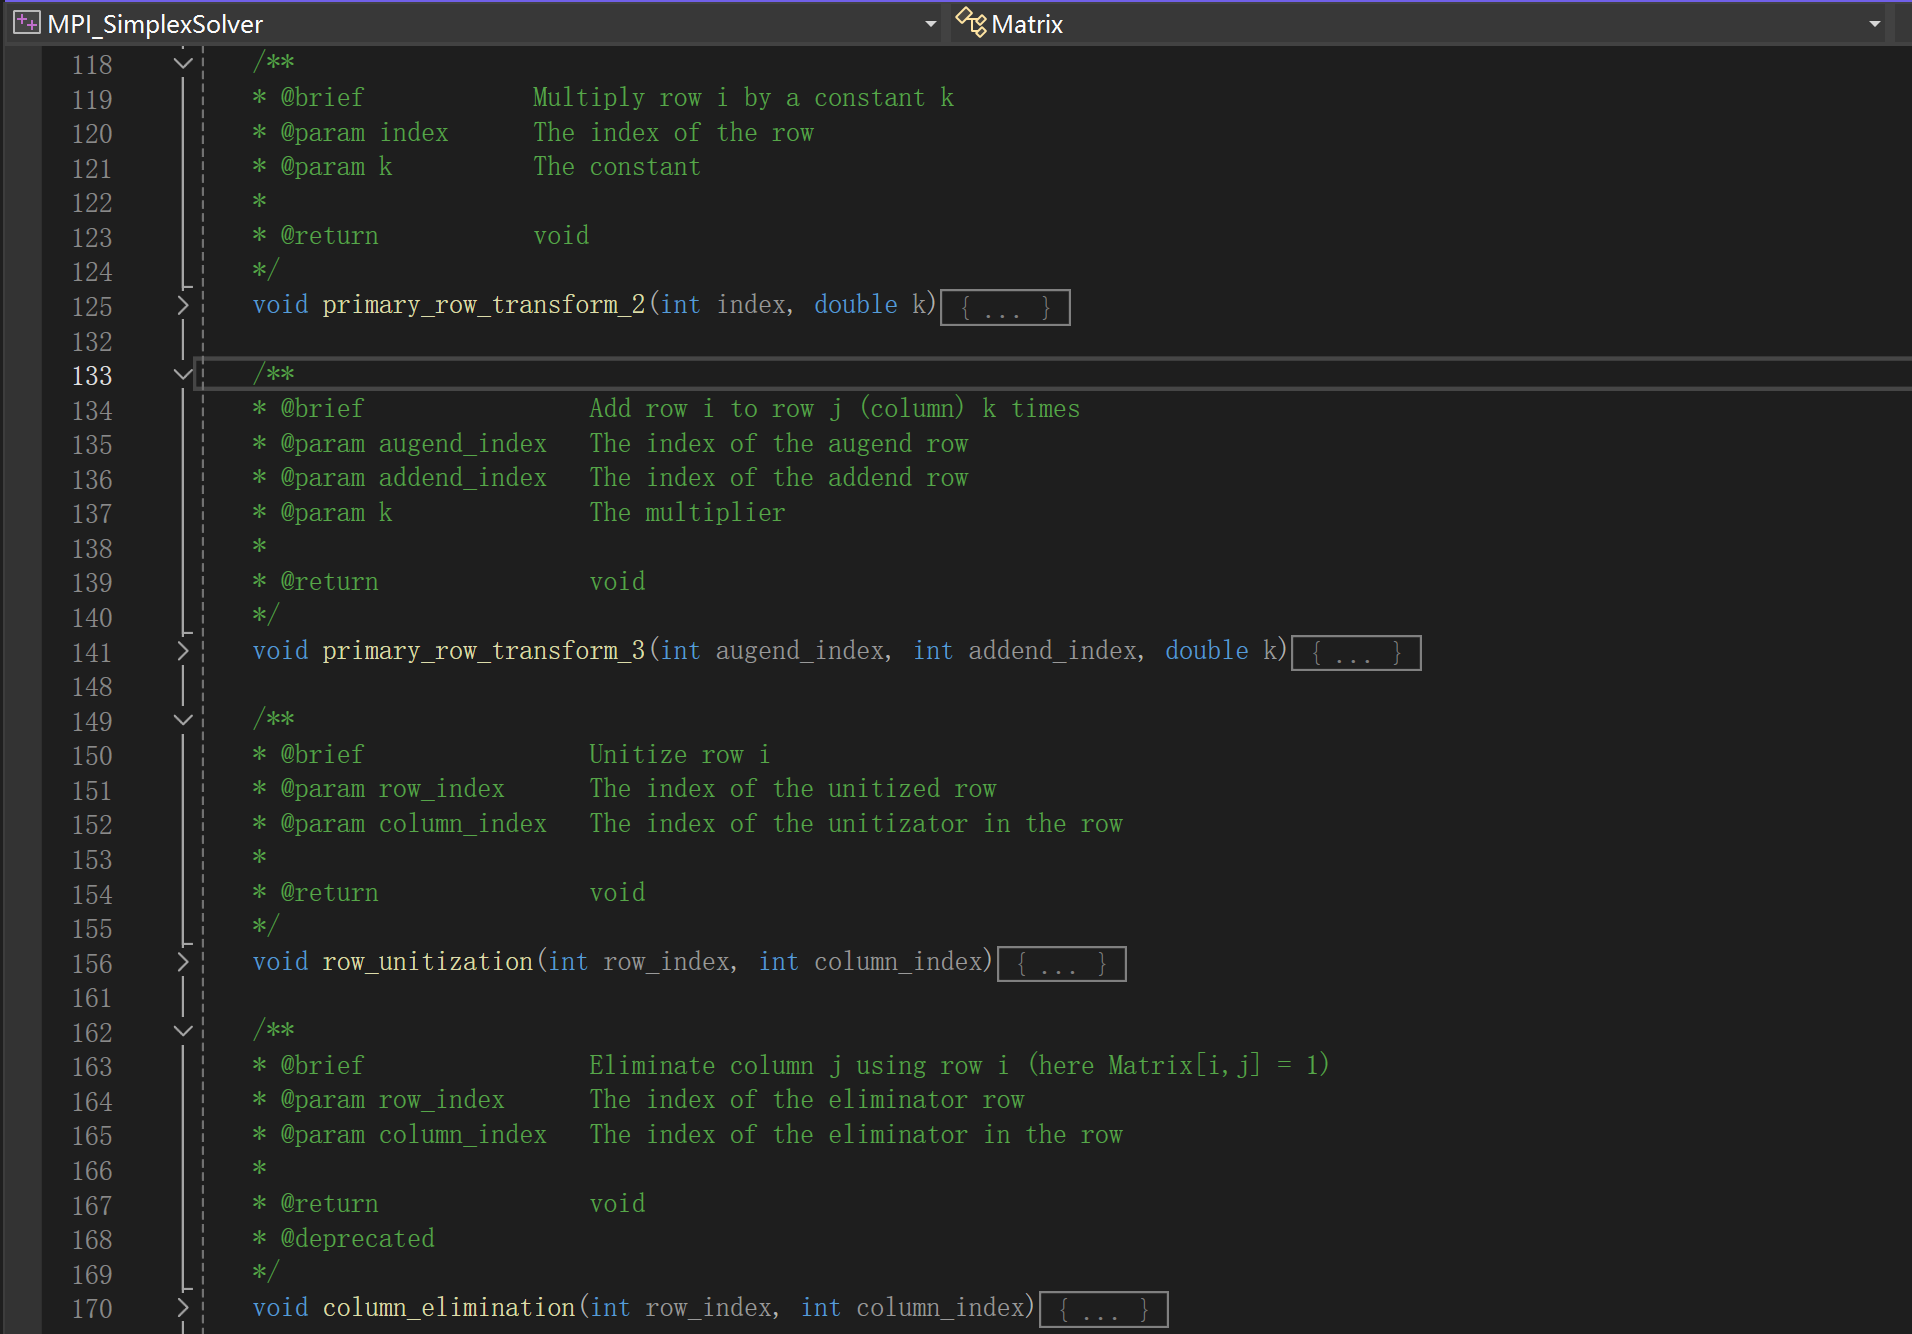
\includegraphics[width=14cm]{Matrix.png}
\end{figure*}
\par
\texttt{Vector}类是介于一维数组与\texttt{Matrix}类间的中介类.
\begin{figure*}[htbp]
    \centering
    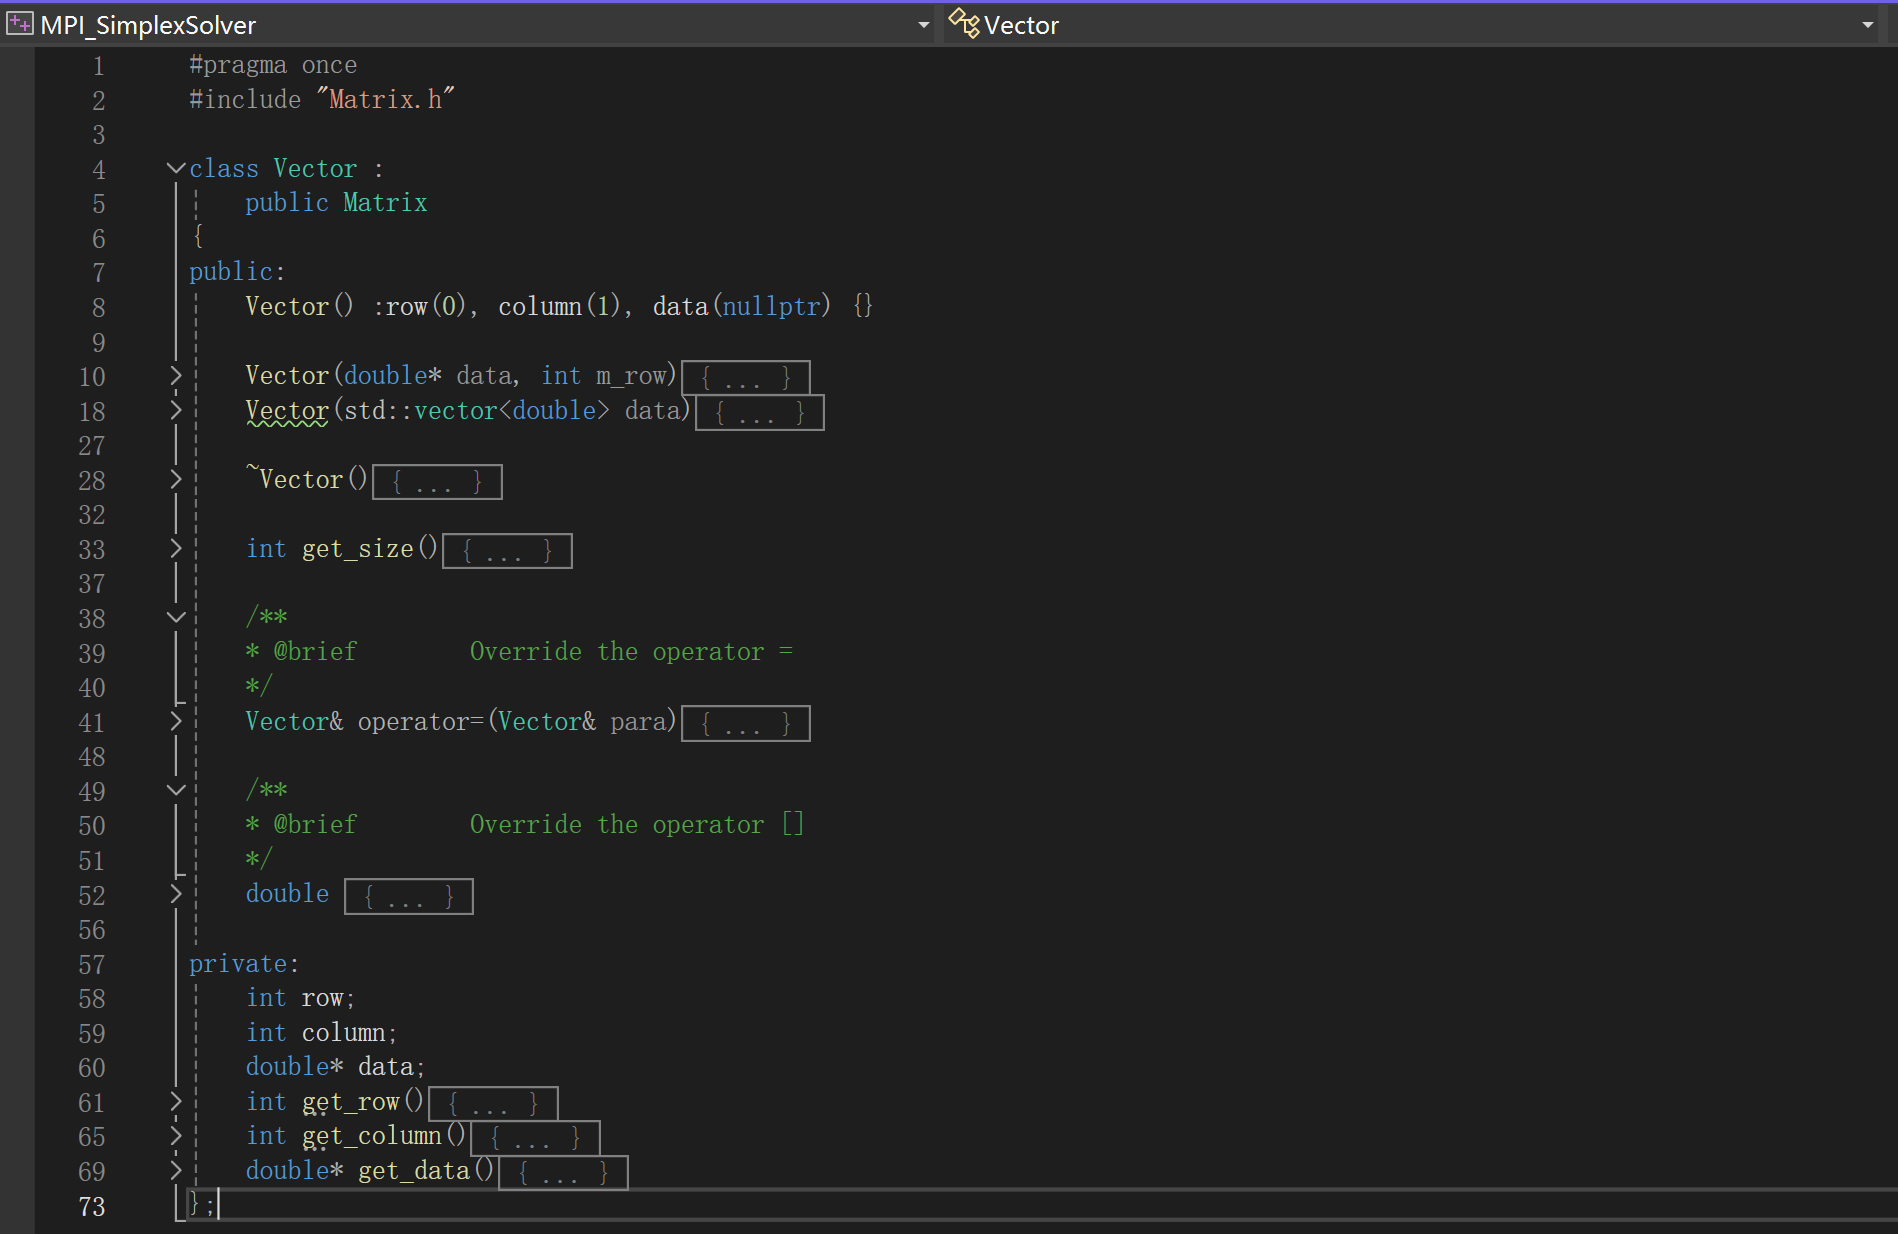
\includegraphics[width=14cm]{Vector.png}
\end{figure*}
\par
\texttt{SimplexSolver}类持有一个\texttt{Matrix}和\texttt{Vector}作为单纯形表和判别数列表, 核心功能函数为单纯形法求解器\texttt{solve()}.
\begin{figure*}[htbp]
    \centering
    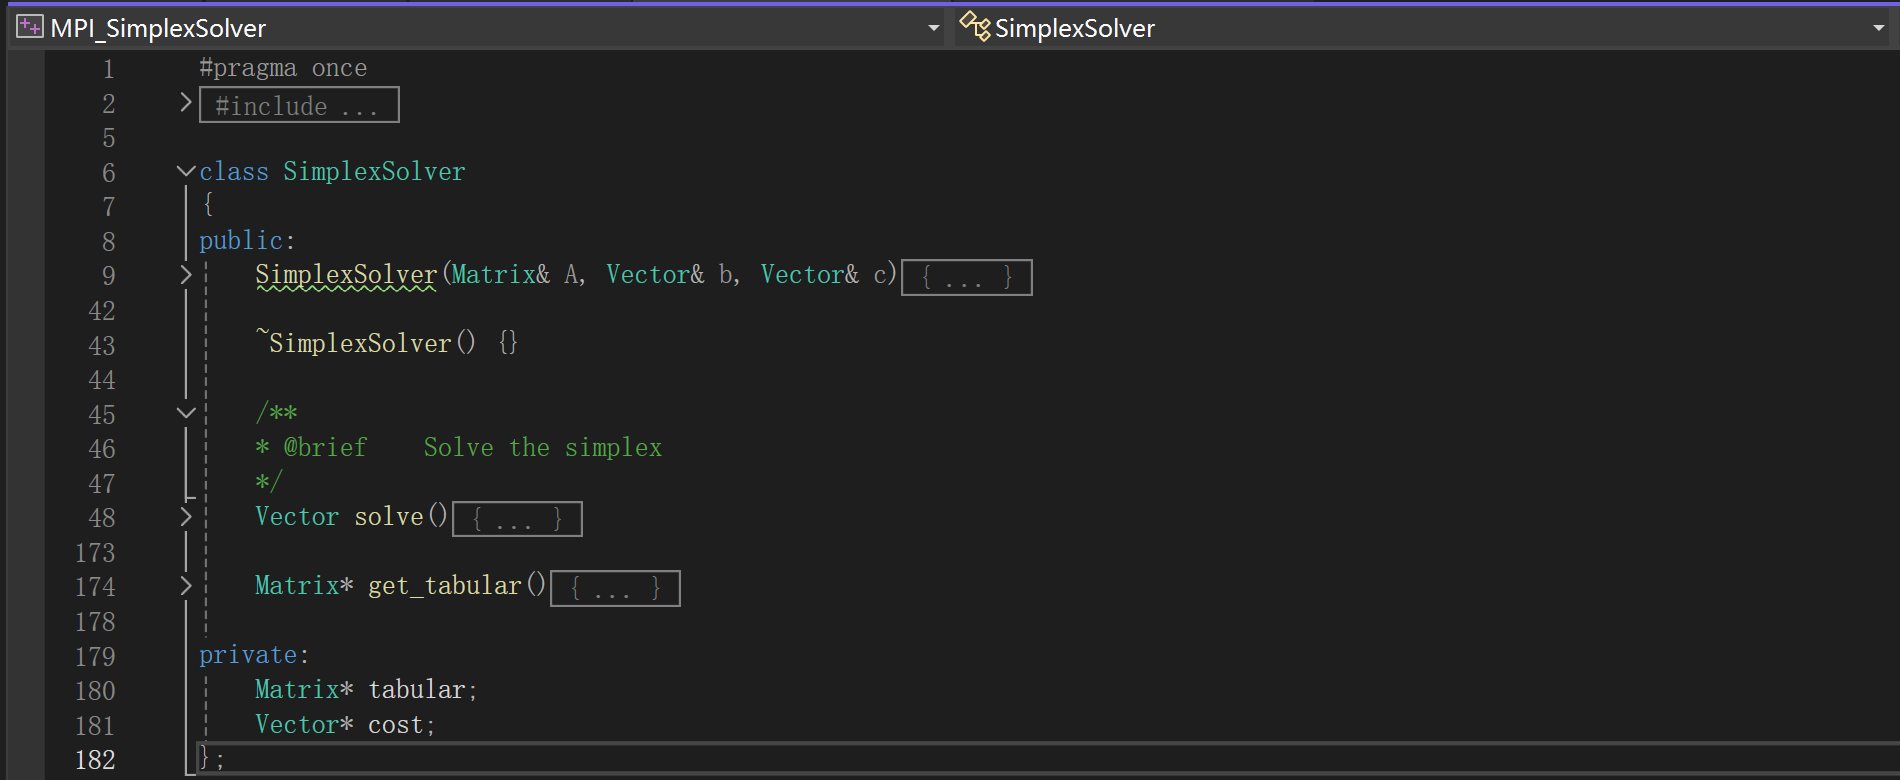
\includegraphics[width=14cm]{SimplexSolver.png}
\end{figure*}
\par
\texttt{MPI\_SimplexSolver}类继承\texttt{SimplexSolver}类, 核心功能函数为\texttt{MPI\_solve\_parallel\_trans()}和\texttt{MPI\_solve\_dir\_search()}, 分别实现了迭代并行和多路径搜索并行计算.
\begin{figure*}[htbp]
    \centering
    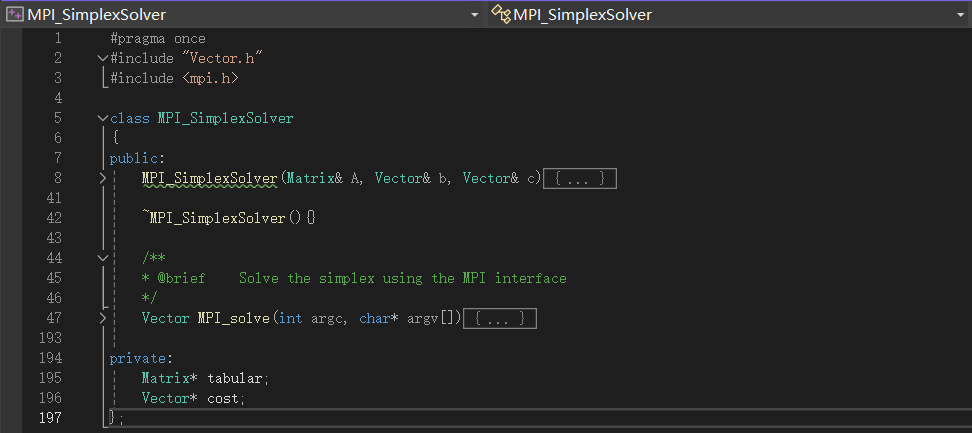
\includegraphics[width=14cm]{MPI_SimplexSolver.png}
\end{figure*}

\section{数值表现}
项目用单线程、\texttt{MPI\_solve\_parallel\_trans()}和\texttt{MPI\_solve\_dir\_search()}分别求解线性规划问题, 其中\texttt{MPI\_solve\_dir\_search()}仅采用变量字典序多路搜索.
\begin{align*}
     & \min f=-2x_1-3x_2                       \\
     & \ \mathrm{s.t.} -x_1 + 2 x_2 + x_3 = 12 \\
     & \qquad 2x_1 + 3x_2 +x_4 = 16            \\
     & \qquad x_1 - x_2 + x_5 = 15             \\
     & \qquad x_i \ge 0 , i=1,2,3,4,5
\end{align*}
重复求解上述问题100000次,运行时间如下.
\begin{table}[h!]
    \begin{center}
        \begin{tabular}{c|c|c}
            单线程   & \texttt{MPI\_solve\_parallel\_trans()} & \texttt{MPI\_solve\_dir\_search()} \\
            \hline
            0.40092s & 0.29572s                               & 0.38109s                           \\
        \end{tabular}
    \end{center}
\end{table}
\texttt{MPI\_solve\_parallel\_trans()}并行加速效果较好, \texttt{MPI\_solve\_dir\_search()}因路径选取为简单字典序选取, 仅有少量加速.
\begin{thebibliography}{5}
    \bibitem{ref1}Richard Marciano, Teodor Rus, Parallel Implementations of the Simplex Algorithm, Proceedings., 2nd Symposium on the Frontiers of Massively Parallel Computation, 10-12, October 1988.
    \bibitem{ref2}Péter Tar, Bálint Stágel, István Maros, Parallel search paths for the simplex algorithm, Central European Journal of Operations Research, (2017) 25:967–984.
\end{thebibliography}

\end{document}